% !TeX spellcheck = de_DE
\clearpage
\section{\ExercisePrefixEmbeddedC WSN---Wide Sensor Network\optional}
\newcommand{\toolWSN}{\textsc{WSN}\xspace}

Ein \toolWSN (Wide Sensor Network) ist ein Netzwerk aus verteilten Sensorknoten. Ziel dieser Aufgabe ist es, das Mikrocontrollerboard um weiteren Mikrocontroller mit WiFi-Schnittstelle zu erweitern, sodass mehrere Boards zusammen ein drahtloses Netzwerk (WLAN) aufspannen können, über welches gemessene Sensordaten an eine zentralen Server-Anwendung gesendet werden können.

Als Erweiterungsmodul nutzen wir das ESP-12E Modul. Dieses wird mit einer modifizierten Version der \href{https://github.com/martin-ger/esp_wifi_repeater}{esp\_wifi\_repeater-Firmware} zum Einsatz. Die Kommunikation zwischen unserem Mikrocontroller und dem ESP-Board wird über UART realisiert.

\begin{enumerate}
	\item Zuerst muss das ESP-Board wie in den beiden Abbildungen zu sehen angeschlossen werden. Dazu sind 4 Leitungen nötig: Masse (GND), Versorgungsspannung (Vcc) und je einmal von Tx (Transmit) zu Rx (Receive) und vice versa.
	
	\begin{minipage}{.5\textwidth}
		\centering
		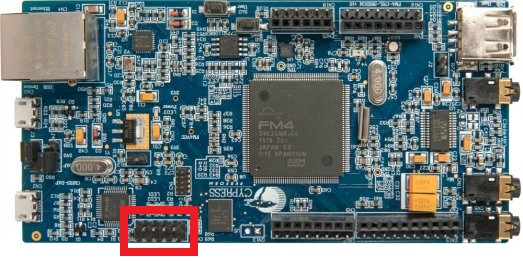
\includegraphics[width=\textwidth]{./05_c/figures/s6e2cc.jpg}
		%\captionof{figure}{Position des Pinheaders auf dem Board}
		%\label{fig:s6e2cc}
	\end{minipage}
	\begin{minipage}{.5\textwidth}		
		\centering
		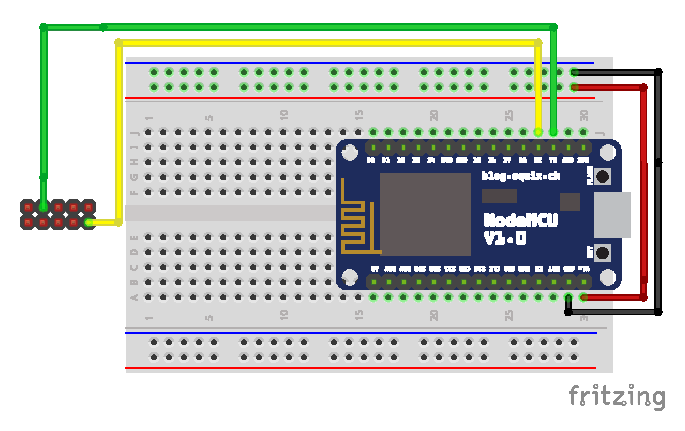
\includegraphics[width=\textwidth]{./05_c/figures/wsnWiring_Steckplatine.pdf}
		%\captionof{figure}{Verkabelung der Platinen}
		%\label{fig:wiring}
	\end{minipage}

	\item Um nun Daten in Form von Zeichenketten zu übertragen, muss zuerst die UART-Schnittstelle initialisiert werden. Dazu reicht es, den header \lstinline|uart_multicon.h| zu includen und die Funktion \lstinline|cpp_initUart3(115200)| aufzurufen. \lstinline|115200| ist die Baudrate mit der die Schnittstelle arbeiten muss.
	
	Zum übertragen von ganzen Zeichenketten, ist es hilfreich zunächst eine Funktion zu implementieren, welche ein einzelnes Zeichen entgegennimmt und überträgt (\zB \lstinline|void writeCharUart3(char c)|). In dieser Funktion muss gewartet werden, solange der Aufruf \lstinline|Mfs_Uart_GetStatus(\&UART3, UartTxEmpty)| nicht \lstinline|TRUE| ergibt. \lstinline|TRUE| ist in diesem Fall ein Makro der Treiberbibliothek, und muss daher genau so verwendet werden. Liefert der Aufruf \lstinline|FALSE| zurück, ist die Schnittstelle bereit um ein einzelnes Zeichen mit dem Aufruf von \lstinline|Mfs_Uart_SendData(\&UART3, c)| zu versenden.
	
	Implementiere nun noch eine Funktion die einen nullterminierten C-String entgegennimmt und durch wiederholte Aufrufe von \lstinline|writeCharUart(char c)| versendet.
	
	Teste deine Funktion, indem du ihr einen Text (\zB \lstinline|"mqtt_pub /Hello World!\r\n"|) übergibst. \lstinline|\r\n| markiert das Ende des Befehls. Auf der Serveranwendung sollte deine Nachricht nun ankommen.
	
	\item Erweitere nun dein Board um einen Sensor, und sende den gemessenen Sensorwert an die Zentrale Serveranwendung. Sende dazu den Befehl \lstinline|"mqtt_wsn <Sensorwert>\r\n"|.
	
	
\end{enumerate}

